\documentclass[aspectratio=169]{beamer}
% Themes ---------------------------------------------------------------------
\usetheme{default}
\usefonttheme{professionalfonts}
% Packages -------------------------------------------------------------------
\usepackage{graphicx}
\usepackage{enumitem}
\usepackage{stmaryrd}
\usepackage[most]{tcolorbox}
\usepackage{booktabs}
\usepackage{import}
\usepackage{adjustbox}
\usepackage{MnSymbol}
\usepackage{fancyvrb}
% Tables ---------------------------------------------------------------------
\renewcommand{\arraystretch}{1.3}
% enumitem -------------------------------------------------------------------
\setlist{itemsep=10pt}
% beamer ---------------------------------------------------------------------
\setbeamerfont{caption}{size=\small}
% Title & author -------------------------------------------------------------
\title{1.2 Setting Up Your Programming Environment}
\subtitle{Getting Started}
\author{Jakob Wells}

\begin{document}
\date{\today}


\begin{frame}
    \titlepage{}
\end{frame}


\begin{frame}[fragile]{Installing Visual Studio Code}
    Download the installer at \href{https://code.visualstudio.com/}{https://code.visualstudio.com/}. \\
    \vspace{10pt}
    \textbf{On macOS} \\
    \begin{enumerate}[label={\arabic*.},itemsep=5pt]
        \item Click the \textbf{Download} link and look for an installer for macOS.
        \item After the file downloads, open it and then drag the Visual Studio Code icon into your \textit{Applications} folder.
    \end{enumerate}
    \vspace{10pt}
    \textbf{On Windows} \\
    \begin{enumerate}[label={\arabic*.},itemsep=5pt]
        \item Click the download link and look for the Windows installer.
        \item After downloading the installer, run the installer and accept all of its defaults.
    \end{enumerate}
\end{frame}


\begin{frame}[fragile]{Installing Visual Studio Code extensions}
    \textbf{View} \(\blacktriangleright\) \textbf{Extensions} \(\blacktriangleright\) \textbf{Search Extensions in Marketplace} \\
    \vspace{15pt}
    \textit{Python} \\
    \href{https://marketplace.visualstudio.com/items?itemName=ms-python.python}{https://marketplace.visualstudio.com/items?itemName=ms-python.python} \\
    \vspace{10pt}
    \textit{Pylance} \\
    \href{https://marketplace.visualstudio.com/items?itemName=ms-python.vscode-pylance}{https://marketplace.visualstudio.com/items?itemName=ms-python.vscode-pylance}
\end{frame}


\begin{frame}[fragile]{Python on macOS (I)}
    Python is already installed on most macOS systems, but it's most likely an outdated version that you won't want to learn on. \\
    \vspace{10pt}
    First, check whether Python is installed on your system.
        \begin{enumerate}[label={\arabic*.},itemsep=5pt]
            \item Open a terminal window by going to \textbf{Applications} \(\blacktriangleright\) \textbf{Utilities} \(\blacktriangleright\) \textbf{Terminal}.
            \item To see which version of Python is installed, enter \textbf{python} with a lowercase \textit{p}.
        \end{enumerate}
    \vspace{10pt}
    You should see output telling you which Python version is installed on your system and a \verb|>>>| prompt where you can start entering Python commands, like this:
    \vspace{5pt}
    \begin{Verbatim}[fontsize=\footnotesize]
$ python
Python 2.7.15 (default, Aug 17 2018, 22:39:05)
[GCC 4.2.1 Compatible Apple LLVM 9.1.0 (clang-902.0.39.2)] on darwin
Type "help", "copyright", "credits", or "license" for more information.
>>>
    \end{Verbatim}
\end{frame}


\begin{frame}[fragile]{Python on macOS (II)}
    This output indicates that Python 2.7.15 is currently the default version installed on this computer.
    Once you've seen this output, press \texttt{CTRL-D} or enter \textbf{exit()} to leave the Python prompt and return to the terminal prompt. \\
    \vspace{10pt}
    To check whether you have Python 3 installed, enter the command \textbf{python3}.
    You'll probably get an error message, meaning you don't have any versions of Python 3 installed. \\
    \vspace{10pt}
    If the output shows you have Python 3.6 or a later version installed, you don't need to do anything.
    If Python 3 isn't installed by default or if you see any version earlier than Python 3.6, you'll need to install the latest version manually. \\
    \vspace{10pt}
    Note that whenever you see the \texttt{python} command, you need to use the \texttt{python3} command instead to make sure you're using Python 3, not Python 2.
\end{frame}


\begin{frame}[fragile]{Installing the latest version of Python}{On macOS}
    You can find a Python installer for your system at \href{https://python.org/}{https://python.org/}. \\
    \vspace{10pt}
    Hover over the \textbf{Download} link, and you should see a button for downloading the latest Python version. \\
    \vspace{10pt}
    Click the button, which should automatically start downloading the correct installer for your system. \\
    \vspace{10pt}
    After the file downloads, run the installer. \\
    \vspace{10pt}
    When you're finished, enter the following at a terminal prompt:
    \vspace{10pt}
    \begin{Verbatim}
$ python3 --version
3.10.6
>>>
    \end{Verbatim}
\end{frame}


\begin{frame}[fragile]{Running Python in a terminal session}{On macOS}
    You can now try running snippets of Python code by opening a terminal session and typing \textbf{python3}.
    Enter the following line in the terminal session:\\
    \vspace{10pt}
    \begin{Verbatim}
>>> print("Hello Python interpreter!")
Hello Python interpreter!
>>>
    \end{Verbatim}
    \vspace{10pt}
    Your message should print directly in the current terminal window.
    Remember that you can close the Python interpreter by pressing \texttt{CTRL-D} or by entering the command \texttt{exit()}.
\end{frame}


\begin{frame}[fragile]{Python on Windows}
    Windows doesn't always come with Python, so you'll probably need to install it, and then install \href{https://code.visualstudio.com/Download}{Visual Studio Code}. \\
    \vspace{10pt}
    First, check whether Python is installed on your system. \\
    \vspace{10pt}
        \begin{enumerate}[label={\arabic*.},itemsep=5pt]
            \item Open a command window by entering \textbf{command} into the Start menu or by holding down the \texttt{SHIFT} key while right-clicking on your desktop and selecting \textbf{Open command window here} from the menu.
            \item In the terminal window, enter \textbf{python} in lowercase.
        \end{enumerate}
    \vspace{10pt}
    If you get a Python prompt (\verb|>>>|) in response, Python is installed on your system.\\
    \vspace{10pt}
    If you see an error message telling you that \texttt{python} is not a recognized command, Python isn’t installed.
\end{frame}


\begin{frame}{Installing Python}{On Windows}
    If Python isn't installed, or if you see a version of Python earlier than Python 3.6, you need to download a Python installer for Windows
    \vspace{10pt}
    \begin{enumerate}[label={\arabic*.},itemsep=5pt]
        \item Go to \href{https://python.org/}{https://python.org/} and hover over the \textbf{Downloads} link.
        \item You should see a button for downloading the latest version of Python.
            Click the button, which should automatically start downloading the correct installer for your system.
        \item After you've downloaded the file, run the installer.
            Make sure you select the option \textbf{Add Python to PATH}, which will make it easier to configure your system correctly.
    \end{enumerate}
\end{frame}


\begin{frame}[fragile]{Running Python in a terminal session (I)}{On Windows}
    Open a command window and enter \textbf{python} in lowercase.
    You should see a Python prompt (\verb|>>>|), which means Windows has found the version of Python you just installed.
    \vspace{10pt}
    \begin{Verbatim}[fontsize=\footnotesize]
C:\> python
Python 3.7.2 (v3.7.2, Dec 23 2018, 23:09:28) [MSC v.1916 64 bit (AMD64)] on win32
Type "help", "copyright", "credits" or "license" for more information.
>>>
    \end{Verbatim}
    \vspace{10pt}
    Enter the following line in your Python session, and make sure you see the output \texttt{Hello Python interpreter!}
    \vspace{10pt}
    \begin{Verbatim}[fontsize=\footnotesize]
>>> print("Hello Python interpreter!")
Hello Python interpreter!
>>>
    \end{Verbatim}
\end{frame}


\begin{frame}[fragile]{Running Python in a terminal session (II)}{On Windows}
    Any time you want to run a snippet of Python code, open a command window and start a Python terminal session. \\
    \vspace{10pt}
    To close the terminal session, press \texttt{CTRL-Z} and then press \texttt{ENTER}, or enter the command \texttt{exit()}.
\end{frame}


% \begin{frame}{Installing Git}
%     \textbf{On macOS} \\
%     To install the latest version of Git, you need to download the installer at \href{https://git-scm.com/download/mac}{https://git-scm.com/download/mac}. \\
%     \vspace{10pt}
%     After the installer downloads, open it and then run the installer with the defaults. \\
%     \vspace{20pt}
%     \textbf{On Windows} \\
%     To install the latest version of Git, you need to download the installer at \href{https://git-scm.com/download/windows}{https://git-scm.com/download/windows}. \\
%     \vspace{10pt}
%     After the installer downloads, open it and then run the installer with the defaults.
% \end{frame}


\begin{frame}[fragile]{Installing Tower}
    \begin{enumerate}[label={\arabic*.},itemsep=5pt]
        \item Download an installer for Tower at \href{https://www.git-tower.com/}{https://www.git-tower.com/}. \\
        \item Click the \textbf{Get Started - It's Free} button.
            The download should begin automatically.
    \end{enumerate}
    \vspace{10pt}
    \textbf{On macOS} \\
        After the file downloads, open it and then drag the Tower icon into your \textit{Applications} folder. \\
    \vspace{20pt}
    \textbf{On Windows} \\
        After downloading the installer run the installer and accept all of its defaults.
        Make sure to choose \textbf{Extract} when asked about installing the embedded git.
\end{frame}


\begin{frame}{Installing embedded git}{On Windows}
    \begin{columns}
        \begin{column}{0.5\textwidth}
            \centering
            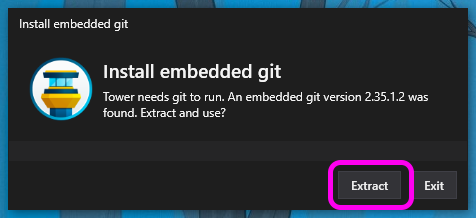
\includegraphics[width=\linewidth]{extract_embedded_git.png}
        \end{column}
    \end{columns}
\end{frame}


\begin{frame}{Registering Tower}{On Windows}
    \begin{columns}
        \begin{column}{0.5\textwidth}
            \centering
            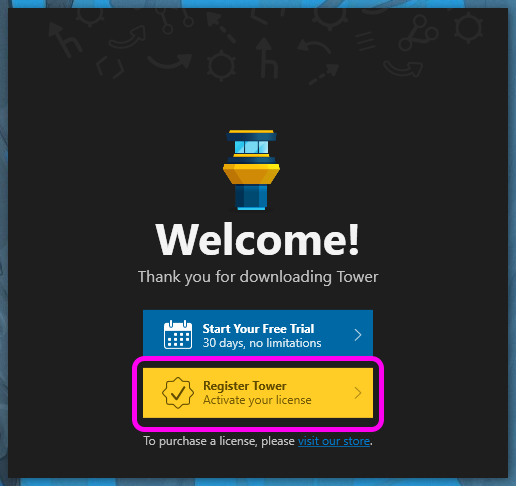
\includegraphics[width=\linewidth]{tower_welcome.png}
        \end{column}
        \begin{column}{0.5\textwidth}
            \centering
            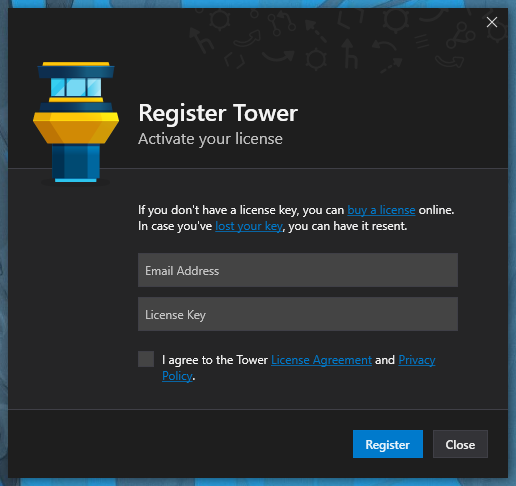
\includegraphics[width=\linewidth]{tower_register.png}
        \end{column}
    \end{columns}
\end{frame}


\begin{frame}{Configuring git}{On Windows}
    \begin{columns}
        \begin{column}{0.5\textwidth}
            \centering
            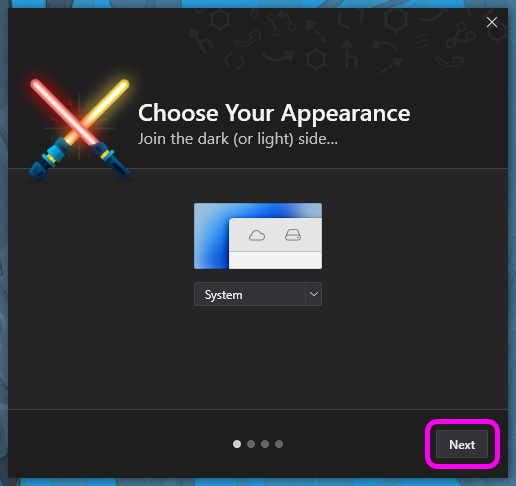
\includegraphics[width=\linewidth]{choose_your_appearance.png}
        \end{column}
        \begin{column}{0.5\textwidth}
            \centering
            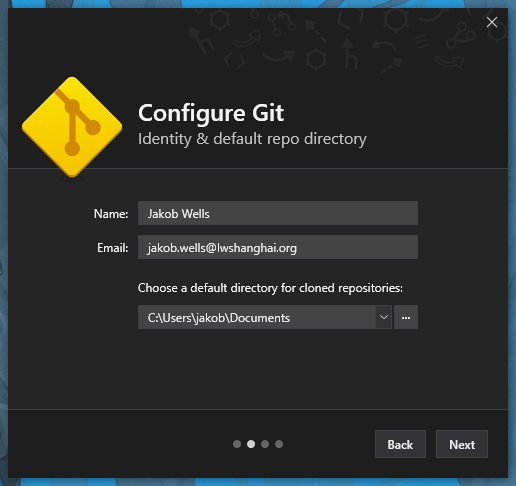
\includegraphics[width=\linewidth]{configure_git.png}
        \end{column}
    \end{columns}
\end{frame}


\begin{frame}{Getting started}{On Windows}
    \begin{columns}
        \begin{column}{0.5\textwidth}
            \centering
            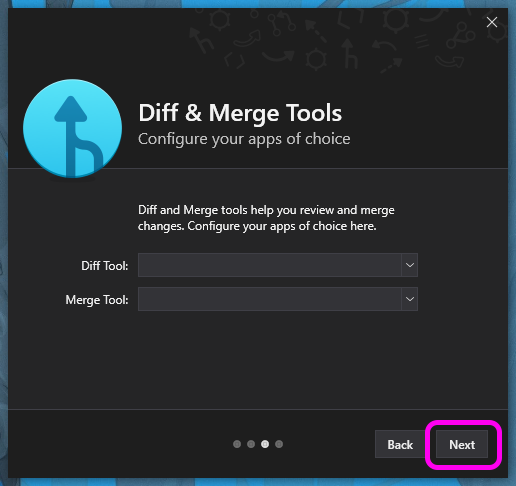
\includegraphics[width=\linewidth]{diff_merge_tools.png}
        \end{column}
        \begin{column}{0.5\textwidth}
            \centering
            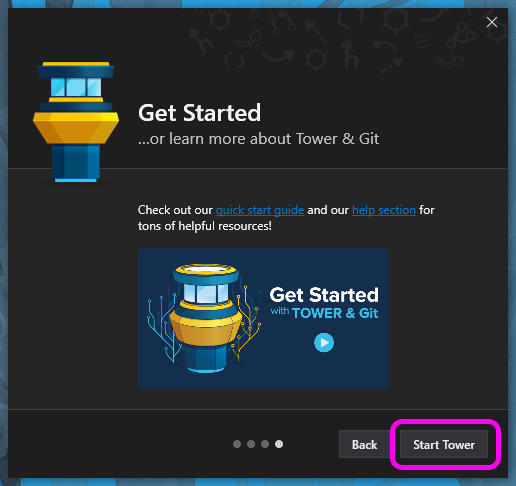
\includegraphics[width=\linewidth]{get_started.png}
        \end{column}
    \end{columns}
\end{frame}


\end{document}
